\documentclass[letterpaper,10pt]{article}
\usepackage{graphicx,amsmath,fancyhdr,times,url,hyperref}
\usepackage[pagewise]{lineno}
\usepackage{upquote}
\oddsidemargin -0in %left margin on odd-numbered pages is 1in + 0in
%%\topmargin -.5in %top margin is 1in -0.5in

\textwidth 6.375in %width of text
\textheight 8.5in % size of page
\setlength{\parindent}{0.0in}
\setlength{\parskip}{7pt}
\renewcommand{\thefootnote}{\fnsymbol{footnote}}

\pagestyle{fancy}
\lhead{EOSC 211-2018}
\rhead{IMAGE LAB-\thepage} 
\chead{Week 3 - Data Structures}
\lfoot{} 
\cfoot{} 
\rfoot{}

\newcounter{lnum}
\newenvironment{abbrevlist}%
  {\begin{list}{(\arabic{lnum})}{\setlength{\leftmargin}{1em}%
               \setlength{\itemindent}{3em}%
               \setlength{\itemsep}{0pt}%
               \setlength{\parsep}{0pt}%
               \setlength{\topsep}{2pt}%
               \usecounter{lnum} } }{\end{list}}
%\linenumbers*[1]

\begin{document}

\section{Introduction}

In this lab we will investigate arrays, do some simple kinds of array
indexing, and make different kinds of plots (read pages 443-456 of the text for info on plotting!). 
We will give you brief code ``snippets'' 
which can be copied. You should learn what is going on by using 
the \verb+help+ command (or the browser-accessible help pages).

At the end of the lab you will
write a short script which will make some plots and this script will be
handed in. Note that this script will require you to put together ideas
you have developed in the earlier parts of the lab.

\begin{figure}[h]
\vspace{10pt}
\centering
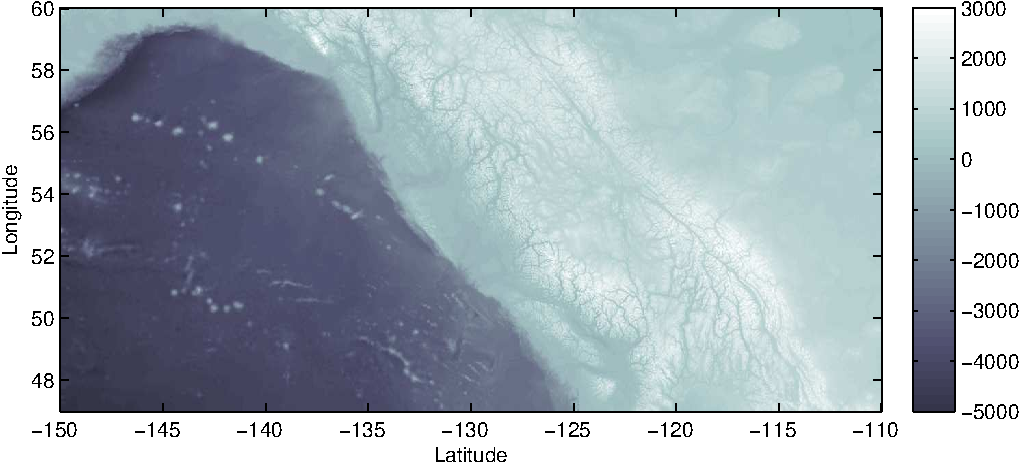
\includegraphics[height=2.5in]{bathy_local-crop.jpg}
\caption{West coast Topography}
\label{f1}
\end{figure}

\section*{Learning goals}
\begin{abbrevlist}
\item  To  download raster image data from the Web and import it into MATLAB
\item  describe the basic parent/child structure in handle graphics
\item  To write short snippets of code that will perform various actions. These include:
\begin{abbrevlist}
\item -displaying raw images and changing the colourmap
\item -retrieving subsections of an array
\item -performing simple mathematical operations on a vector
\item -displaying a contour plot
\item -using handles, get and set property/value pairs to customize graphics.
\end{abbrevlist}
\item  To build up a larger program by continually modifying a small 'starter' program.
\item  To write a short program that performs specified actions.  

\end{abbrevlist}

{\bf NOTE: When people run into problems in this lab, it is generally because they have skipped ahead of
early sections, or failed to answer questions in some part because 
they seem ``too easy''.}

\newpage
\section{Ocean Colour}

There is a vast quantity of earth sciences data online. Many servers
provide a web interface to plot the data, and often there is also a way
to download the actual data. Open your web browser to the NASA Ocean Colour Web site 
(\url{https://oceancolor.gsfc.nasa.gov})
and go to the ``Data'' link at the top of the left hand menu bar, then go to the ``LEVEL 3 Browser'' link.  Thumbnail images will appear with 4 pulldown menus.  Leave the leftmost one set to its default (``standard''),
and the 3rd one at ``monthly''.

The major products of  ocean colour satellites (CZCS, OCTS, SeaWiFS, MODIS, and now VIIRS/SNPP satellites) are 
chlorophyll (a measure of phytoplankton biomass) and sea-surface temperature (SST). Look around and find a nice SNPP VIIRS Chlorophyll or
Sea Surface Temperature image at some interesting date (month of your birthday?). {\bf One of the MONTHLY images
tends to work better in this lab because you can easily see the difference
between land and water regions}.

Select the 9km resolution (right hand menu bar), and click on the thumbnail
to open a rather large image in your browser. Right-click on
the image to save it to your disk (if you accidentally click near the lower left or right you will be asked if you want 
a binary file with a .nc extension - this is NOT what you want).

Now, load and display the file using
\begin{verbatim}
[A,CMAP]=imread('your_filename.png'); % use your file name here.
image(A);
xlabel('Column Index');
ylabel('Row index');
colormap(CMAP)
\end{verbatim}

The matrix \verb+A+ is pretty large (how large? - check using the \verb+size+ function, or look in the
Workspace window).
Points on the same latitude are in the same row (first dimension), and 
points with the same longitude are in the same column (2nd dimension). 
But what does the data in \verb+A+ actually represent? Where do those greens and blues come from?

All colours on the computer screen are generated as
a combination of only 3 colours - red, green, and blue (RGB)\footnote{other colour models such as HSV and CMYK also exist}. We can represent
any colour as some combination of the 3, each with a fraction between 0 and 1  - say, 
by a 3-element vector \verb+[.3 .6 .2]+
which means 30\% red, 60\% green, and 20\% blue. Black would be \verb+[0 0 0]+ and
white is \verb+[1 1 1]+. The $256\times 3$ variable \verb+CMAP+ holds 256 of these colours,
and the values in \verb+A+, which are between 0 and 255 (inclusive) are an index into this color
table. The \verb+colormap()+ function sets the colours to be used in the current figure.
To see the colours plotted out by their index in a horizontal 'colour bar', type:
\begin{verbatim}
figure(2)
image(uint8(0:255))
colormap(CMAP);
\end{verbatim}
The ``:" is a special OPERATOR which is very useful in MATLAB.  We saw it in class and lab last week, but type \verb+help colon+ to 
understand what it does if you've forgotten.
 
You can look at smaller areas by ZOOMING in and out using the GUI controls at the top of the
figure. Instead, let us make a figure of a smaller area by {\bf extracting a subset} of the whole global
image. In the plot, the row and column indexes are
marked on the axes. So, for example, we can show only the western North Atlantic in a new figure window using

\begin{verbatim}
WNA=A(300:650,1350:1700);
figure(3)
image(WNA);
colormap(CMAP);
\end{verbatim}

(Why those numbers?). Now extract and display an image of the ocean near Vancouver, instead of the western
North Atlantic. {Hint: think about what rows and columns you need}.   Notice what happens if you don't include the line \verb+colormap(CMAP)+ when you make your figure.

Now you know how to pull out pieces of an image. But this isn't just an image, it's actually
geographic data. It would be nice if
we could have axes labelled in longitude and latitude. 

How is this done? By ``telling'' the \verb+image+ command what the x- and y- values of
the rows and columns in the matrix are, instead of letting it default to labelling things by the row and column
indexes. For the x-axis, we can make a vector with the same
number of elements as there are columns in \verb+A+. The first element of the vector will contain 
the numerical value of the longitude of the westernmost column, and the last element will
contain the longitude of the easternmost. Similarly, for the y-axis we need a vector containing
the numerical latitudes of all rows, with the first element giving the latitude of the northernmost
row.

 
\begin{verbatim}
nA=size(A);
lat=  90-180*[1:nA(1)]/nA(1);   
lon=-180+360*[1:nA(2)]/nA(2);
image(lon,lat,A);
xlabel('Longitude');
ylabel('Latitude');
% The next line changes the direction of the y axis so numbers increase upwards 
set(gca,'ydir','normal');
\end{verbatim}

What is happening in the first line? The \verb+size+ function RETURNS an array of values - the
number of rows and columns of \verb+A+ - and assigns these values to the $1\times 2$
variable
\verb+nA+. How about the next two lines? What numbers end up in
the \verb+lat+ and \verb+lon+ variables?

Also, what's up with that line with the \verb+set()+ command?  We will talk about \verb+set()+ again later in the term when we look at making more sophisticated plots, but for now here's a summary:

\fbox{\parbox{6in}{In MATLAB, figures are organized as OBJECTS, which can be addressed with a HANDLE. Each
object can have PROPERTIES and CHILDREN. Properties affect the look-and-feel of an object.
Children are other objects, associated with the current object (huh?).
\vspace{10pt}

The children of a figure window are the different
subplots in it, and the children of individual subplots will be the lines and images displayed on it.
\vspace{10pt}

Properties of a figure include the colour of the window (default gray). Properties of a
subplot include the axis limits, and the ticklabels. Properties of a line include its colour and thickness.

\vspace{10pt}

Properties are accessed using property/value pairs - a NAME, followed by its VALUE.
The  {\tt set} command lets you change properties. {\tt gca} is a function returning the
HANDLE of the ``current axis'' (get-current-axis). {\tt ydir} is a property of the axis, and
{\tt 'normal'} is a string telling which direction you want y-axis values to increase upwards (the default
with {\tt image} is to increase downwards).

\vspace{10pt}
{\tt get(gca) }  tells you the current setting of axes properties

{\tt set(gca) }  tells you the different options for axes properties
}}

Now make a plot of the Vancouver area with the correct longitude and latitudes on the axes ({\bf Hint:
you have to extract subsections of the \verb+lat+ and \verb+lon+ arrays as well}).
Vancouver is near 49$^\circ$N, 123$^\circ$W (or -123$^\circ$E).

You can provide a title for the plot using the \verb+title+ function, and labels for
the x and y axes using \verb+xlabel+ and \verb+ylabel+. Do so. It is good practice to
properly label axes and you should always do so in this course (especially when handing
things in!). Strictly speaking we also probably want to label longitudes as E and W
rather than positive and negative but this is a more advanced topic.

%\newpage

\section{Global Topography}

The png image we used in the last part was already {\it scaled}, so e.g. if you chose a chlorophyll map, the real world values with units of concentration between 0
and 30~mg~m$^{-3}$ had already been
turned into integers between 0 and 255. To do any science with these maps we would need to
refer to the colorbar that showed the original maximum and minimum values 
(see this bar at the bottom of the L3 data browser). In this section we will deal
with {\it unscaled} data.

First, we will examine the topography in our part of the world. Clear the workspace using the \verb+clear+
command.
Now download the data file
\verb+Bathyfile.mat+ from the course web site and read it into MATLAB (recall loading \verb+.mat+ files in the
last lab). Note that you have one new variable, the STRUCTURE \verb+bath+. What are its
subfields?

\verb+bath.height+ contains a matrix of elevations (heights above sea level), not RGB values.
How will matlab show this? The easiest way is to use a variant of \verb+image+:
\begin{verbatim}
figure(1)
imagesc(bath.long,bath.lat,bath.height);
xlabel('Longitude');
ylabel('Latitude');
colorbar;
set(gca,'ydir','normal');
\end{verbatim}

The default colourmap in MATLAB versions 2014a and earlier is \verb+jet+ which goes from dark blue for lowest values to dark red
for largest values. In MATLAB versions 2014b and later the default is \verb+parula+ which goes from dark blue for the lowest values to yellow for the highest values.  Try some others, e.g. the \verb+hsv+ colormap:
\begin{verbatim}
colormap(hsv)
\end{verbatim}
and try switching between \verb+parula+ and \verb+jet+ and see if you think MATLAB should have changed the default!
(MATLAB also has other predefined colourmaps, see if you can find and use them).

The \verb+imagesc+ function SCALES the data values into the range of colourmap indices.
We can modify this mapping with the \verb+caxis+ function. For example, this will
show only the mountains:
\begin{verbatim}
caxis([0 4200]);
\end{verbatim}

What are the actual heights in different places? What we want to do here is to a)
find the row/column INDEX of a desired location, and b) extract that value from
the array. The \verb+ginput+ function lets you use the mouse to get a location on
the figure axes.  \verb+ginput+ works with row and column numbers NOT with real-world x,y or in this 
case longitude and latitude values.  So first make a figure showing the elevations with just row numbers and column numbers plotted.
Notice that as before row numbers increase from top to bottom .

\begin{verbatim}
  figure(2)
  imagesc(bath.height);
\end{verbatim}

Now cut and paste this snippet into the command window.

\begin{verbatim}
% Pick some points and label them   
  [I,J]=ginput(1);
  I=round(I);
  J=round(J);
  bath.height(J,I)
  text(I,J,num2str(bath.height(J,I)));
\end{verbatim}
  
What does it do? (Hint: Click a mouse button when the mouse
is over the image). Now go through this line by line and decide what is going on.  What is contained in the variables \verb+I, J, bath.height(I,J)+? We will see more of \verb+ginput+ in future labs. What matlab code would you write to get the latitude and longitude of the point that you have clicked?  Check your answer looks about right by looking at Figure 1.  


Finally, extract a row from the grid of elevations, and make a line plot
\begin{verbatim}
plot(bath.long,bath.height(256,:));
\end{verbatim}
What latitude is this row? Put it in a title and add x-axis and y-axis labels. Lastly, add a zero line to your plot to show where sea-level is. To do this you'll first need to turn on the hold to prevent the figure from being redrawn, and then draw a line at the zero-level:
\begin{verbatim}
hold on;
plot([bath.long(1) bath.long(end)], [0 0], 'k')
\end{verbatim}
Experiment to see what happens if you don't include the \verb:hold on: command, or if you replace \verb:'k': with \verb:'r':.

\section{Ocean Salinity}

First, \verb+clear+ the workspace. Then, get the file \verb+salt.txt+ from the course website. Look at it in an editor. It is made up of columns of numbers, some
of which are \verb+NaN+. You can load this text table into a matrix S as follows:
\begin{verbatim}
S=load('salt.txt');
\end{verbatim}

\verb+S+ has 34 rows and 42 columns, organized into a table. 
Columns \verb+2:42+ of row 1 are the longitudes of data below them in the same column.
Rows \verb+2:34+ of column 1 are the depths of the data in the rest of the row. 
Columns \verb+2:42+ of rows
\verb+2:34+ are salinity values (in grams per kg seawater), one for each particular depth and longitude, at a latitude of $51.5^{\circ}$N. 

Extract
the depth, longitude, and salinity values into subfields of a structure \verb+sal+ so that

\verb+plot(sal.salinity,sal.depth)+ shows depth profiles of salinity, and 

\verb+plot(sal.long,sal.salinity)+ shows curves of salinity at different depths as a function of longitude.

{\bf NOTE:} that this is a special case of plotting.  We talked last week about the fact that typically when plotting two quantities x and y, the arrays \verb+x, y+ must have the same dimensions.  This is obviously an exception because \verb+sal.longitude, sal.depth and sal.salinity+ do not have the same dimensions but MATLAB has still produced a plot that makes sense. What do you think has happened here?  We will see more of this later in the course.

Next, make a contour map of this data using
\begin{verbatim}
contour(sal.long,sal.depth,sal.salinity,[31.5:.1:35]);
\end{verbatim}
or (perhaps more clear)
\begin{verbatim}
contourf(sal.long,sal.depth,sal.salinity,[31.5:.1:35]);
\end{verbatim}

What does the last argument to the \verb+contour+ command do?  Notice that the contours don't extend over the whole region of your plot.  This is because \verb+sal.salinity+ contains \verb+NaN+ in some elements (why do you think this is in this problem?) and so MATLAB does not attempt to draw contours in these regions.  

Finally, 
add the curve of elevations you plotted at the end of the last section using
\begin{verbatim}
plot(bath.long,bath.height(256,:));
\end{verbatim}
Since you cleared the workspace, you will have to reload \verb+Bathyfile.mat+ before this works.
Also, you will have to use the  \verb+hold on+ command to prevent the \verb+plot+
function from erasing the contour plot. You can manually set the axis limits
using the \verb+axis+ command, or using \verb+ylim+ and \verb+xlim+ if you get it wrong \verb+axis auto+ may be useful in tracking
down the problem.

\section{To Hand In by 4:00 pm on Friday, September 21st}

You {\bf NEED NOT} hand in {\bf EVERYTHING} you have done. Instead, you must gather together the {\bf relevant} bits of code
you have already written and
write and hand in a script file called (exactly) \verb+lab3.m+ which will do EXACTLY the following (no less and no more):
\begin{abbrevlist}
\item load the file \verb+Bathyfile.mat+  
\item load the file \verb+salt.txt+, and extract its data into a structure
\item Make a plot with axis labels and a title showing contours of salinity (as a function of longitude and depth).  Use \verb+contourf+
\item Overplot on it lines showing bathymetry (heights and depths) as a function of longitude at $48^{\circ}$N, $51.5^{\circ}$N,
and $55^{\circ}$N latitudes.
\item \verb+lab3.m+ should also contain the following (and exactly the following)
lines of working code:
\begin{verbatim}
partner.name='YYYYYY';
Time_spent= XX;
\end{verbatim}
where YYYYYY (string) is the person with whom you were paired in the labs (remember to put single
quotes around the name) and 
and XX (number) is your estimate of the {\bf number of hours} spent both in the scheduled lab 
period and outside it to complete this lab.

\end{abbrevlist}
It is important to follow these instructions because your code will be semi-automatically ``run-tested'' by a program that
expects your code to follow these specifications.

Hint: To make sure your script works after adding the partner info - {\bf save}, quit Matlab, restart Matlab, and type \verb+lab3+ at the command line.

%%\section{PS}


%%\begin{verbatim}
%% set(gca,'xtick',[-150:5:-110],'xticklabel',{'150W','145W','140W','135W','130W',...
%%                                             '125W','120W','115W','110W'});
%% set(gca,'ytick',[48:2:60],'yticklabel',{'48N','50N','52N','54N','56N','58N','60N'});
%%\end{verbatim}




\end{document}



